\documentclass[tikz,border=5pt]{standalone}
\usepackage{times}
\usepackage{amsmath,amssymb}
\usetikzlibrary{positioning,fit,arrows.meta,backgrounds,shapes.geometric,calc,shadows,decorations.pathreplacing}

\begin{document}
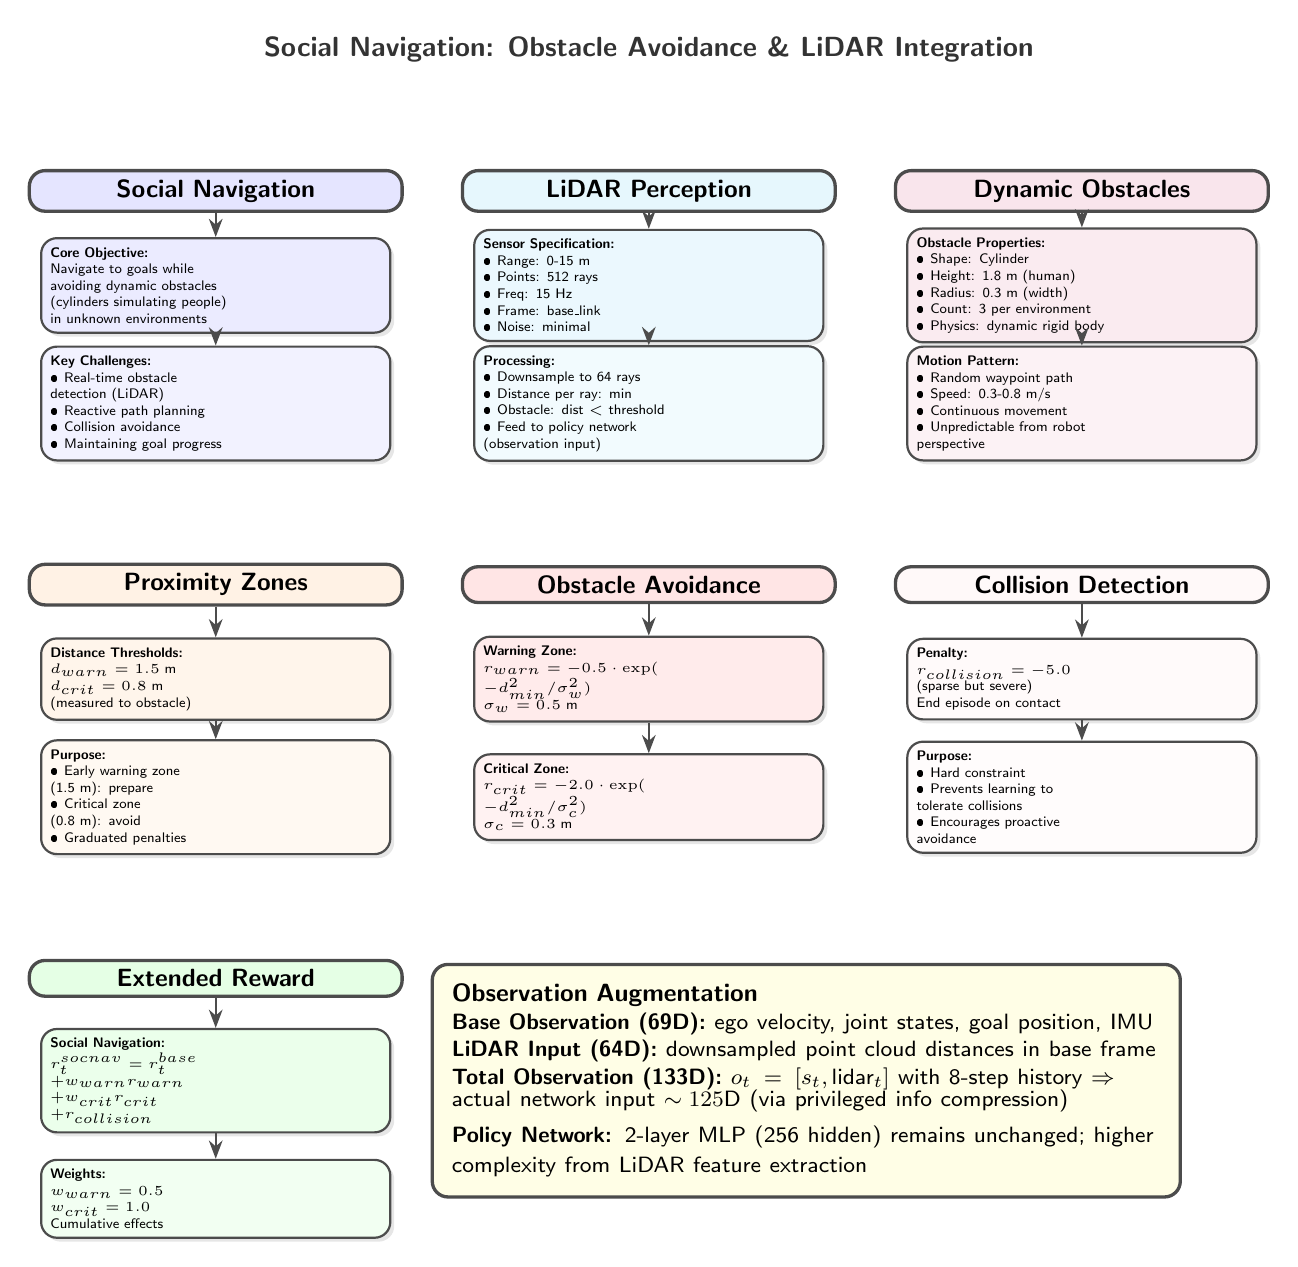
\begin{tikzpicture}[
    node distance=1.0cm and 1.3cm,
    box/.style={
        draw=black!70,
        rounded corners=2mm,
        fill=white,
        thick,
        font=\sffamily\small,
        align=center,
        drop shadow={opacity=0.2, shadow xshift=0.05cm, shadow yshift=-0.05cm}
    },
    header/.style={
        font=\sffamily\bfseries\normalsize,
        color=black!80
    },
    formula/.style={
        font=\ttfamily\footnotesize,
        color=black!70
    },
    arrow/.style={->, >=Stealth, thick, color=black!70},
    label/.style={font=\sffamily\tiny, color=black!60}
]

% ============================================================
% TITLE
% ============================================================
\node[header] at (7.5, 13.8) {Social Navigation: Obstacle Avoidance \& LiDAR Integration};

% ============================================================
% SOCIAL NAV PRINCIPLES (TOP-LEFT)
% ============================================================
\node[draw=black!70, rounded corners=2mm, fill=blue!10, very thick, text width=4.5cm, align=center, font=\sffamily\small] (socnav_header) at (2.0, 12.0) {\textbf{Social Navigation}};

\node[box, fill=blue!8, text width=4.2cm, font=\sffamily\tiny, align=left] (socnav_principle) at (2.0, 10.8) {
\textbf{Core Objective:}\\
Navigate to goals while\\
avoiding dynamic obstacles\\
(cylinders simulating people)\\
in unknown environments
};

\node[box, fill=blue!5, text width=4.2cm, font=\sffamily\tiny, align=left] (socnav_challenge) at (2.0, 9.3) {
\textbf{Key Challenges:}\\
• Real-time obstacle\\
  detection (LiDAR)\\
• Reactive path planning\\
• Collision avoidance\\
• Maintaining goal progress
};

\draw[arrow] (socnav_header) -- (socnav_principle);
\draw[arrow] (socnav_principle) -- (socnav_challenge);

% ============================================================
% LIDAR SENSING (TOP-CENTER)
% ============================================================
\node[draw=black!70, rounded corners=2mm, fill=cyan!10, very thick, text width=4.5cm, align=center, font=\sffamily\small] (lidar_header) at (7.5, 12.0) {\textbf{LiDAR Perception}};

\node[box, fill=cyan!8, text width=4.2cm, font=\sffamily\tiny, align=left] (lidar_spec) at (7.5, 10.8) {
\textbf{Sensor Specification:}\\
• Range: 0-15 m\\
• Points: 512 rays\\
• Freq: 15 Hz\\
• Frame: base\_link\\
• Noise: minimal
};

\node[box, fill=cyan!5, text width=4.2cm, font=\sffamily\tiny, align=left] (lidar_process) at (7.5, 9.3) {
\textbf{Processing:}\\
• Downsample to 64 rays\\
• Distance per ray: min\\
• Obstacle: dist $<$ threshold\\
• Feed to policy network\\
(observation input)
};

\draw[arrow] (lidar_header) -- (lidar_spec);
\draw[arrow] (lidar_spec) -- (lidar_process);

% ============================================================
% OBSTACLE REPRESENTATION (TOP-RIGHT)
% ============================================================
\node[draw=black!70, rounded corners=2mm, fill=purple!10, very thick, text width=4.5cm, align=center, font=\sffamily\small] (obs_header) at (13.0, 12.0) {\textbf{Dynamic Obstacles}};

\node[box, fill=purple!8, text width=4.2cm, font=\sffamily\tiny, align=left] (obs_spec) at (13.0, 10.8) {
\textbf{Obstacle Properties:}\\
• Shape: Cylinder\\
• Height: 1.8 m (human)\\
• Radius: 0.3 m (width)\\
• Count: 3 per environment\\
• Physics: dynamic rigid body
};

\node[box, fill=purple!5, text width=4.2cm, font=\sffamily\tiny, align=left] (obs_motion) at (13.0, 9.3) {
\textbf{Motion Pattern:}\\
• Random waypoint path\\
• Speed: 0.3-0.8 m/s\\
• Continuous movement\\
• Unpredictable from robot\\
  perspective
};

\draw[arrow] (obs_header) -- (obs_spec);
\draw[arrow] (obs_spec) -- (obs_motion);

% ============================================================
% PROXIMITY ZONES (MIDDLE-LEFT)
% ============================================================
\node[draw=black!70, rounded corners=2mm, fill=orange!10, very thick, text width=4.5cm, align=center, font=\sffamily\small] (prox_header) at (2.0, 7.0) {\textbf{Proximity Zones}};

\node[box, fill=orange!8, text width=4.2cm, font=\sffamily\tiny, align=left] (prox_zones) at (2.0, 5.8) {
\textbf{Distance Thresholds:}\\
$d_{warn} = 1.5$ m\\
$d_{crit} = 0.8$ m\\
(measured to obstacle)
};

\node[box, fill=orange!5, text width=4.2cm, font=\sffamily\tiny, align=left] (prox_purpose) at (2.0, 4.3) {
\textbf{Purpose:}\\
• Early warning zone\\
  (1.5 m): prepare\\
• Critical zone\\
  (0.8 m): avoid\\
• Graduated penalties
};

\draw[arrow] (prox_header) -- (prox_zones);
\draw[arrow] (prox_zones) -- (prox_purpose);

% ============================================================
% OBSTACLE PROXIMITY REWARD (MIDDLE-CENTER)
% ============================================================
\node[draw=black!70, rounded corners=2mm, fill=red!10, very thick, text width=4.5cm, align=center, font=\sffamily\small] (obsavoid_header) at (7.5, 7.0) {\textbf{Obstacle Avoidance}};

\node[box, fill=red!8, text width=4.2cm, font=\sffamily\tiny, align=left] (obsavoid_formula) at (7.5, 5.8) {
\textbf{Warning Zone:}\\
$r_{warn} = -0.5 \cdot \exp($\\
$-d_{min}^2 / \sigma_w^2)$\\
$\sigma_w = 0.5$ m
};

\node[box, fill=red!5, text width=4.2cm, font=\sffamily\tiny, align=left] (obsavoid_behavior) at (7.5, 4.3) {
\textbf{Critical Zone:}\\
$r_{crit} = -2.0 \cdot \exp($\\
$-d_{min}^2 / \sigma_c^2)$\\
$\sigma_c = 0.3$ m
};

\draw[arrow] (obsavoid_header) -- (obsavoid_formula);
\draw[arrow] (obsavoid_formula) -- (obsavoid_behavior);

% ============================================================
% COLLISION PENALTY (MIDDLE-RIGHT)
% ============================================================
\node[draw=black!70, rounded corners=2mm, fill=pink!10, very thick, text width=4.5cm, align=center, font=\sffamily\small] (coll_header) at (13.0, 7.0) {\textbf{Collision Detection}};

\node[box, fill=pink!8, text width=4.2cm, font=\sffamily\tiny, align=left] (coll_penalty) at (13.0, 5.8) {
\textbf{Penalty:}\\
$r_{collision} = -5.0$\\
(sparse but severe)\\
End episode on contact
};

\node[box, fill=pink!5, text width=4.2cm, font=\sffamily\tiny, align=left] (coll_purpose) at (13.0, 4.3) {
\textbf{Purpose:}\\
• Hard constraint\\
• Prevents learning to\\
  tolerate collisions\\
• Encourages proactive\\
  avoidance
};

\draw[arrow] (coll_header) -- (coll_penalty);
\draw[arrow] (coll_penalty) -- (coll_purpose);

% ============================================================
% EXTENDED REWARD FUNCTION (BOTTOM-LEFT)
% ============================================================
\node[draw=black!70, rounded corners=2mm, fill=green!10, very thick, text width=4.5cm, align=center, font=\sffamily\small] (ext_reward_header) at (2.0, 2.0) {\textbf{Extended Reward}};

\node[box, fill=green!8, text width=4.2cm, font=\sffamily\tiny, align=left] (ext_reward_formula) at (2.0, 0.7) {
\textbf{Social Navigation:}\\
$r_t^{socnav} = r_t^{base}$\\
$+ w_{warn} r_{warn}$\\
$+ w_{crit} r_{crit}$\\
$+ r_{collision}$
};

\node[box, fill=green!5, text width=4.2cm, font=\sffamily\tiny, align=left] (ext_reward_weights) at (2.0, -0.8) {
\textbf{Weights:}\\
$w_{warn} = 0.5$\\
$w_{crit} = 1.0$\\
Cumulative effects
};

\draw[arrow] (ext_reward_header) -- (ext_reward_formula);
\draw[arrow] (ext_reward_formula) -- (ext_reward_weights);

% ============================================================
% OBSERVATION AUGMENTATION (BOTTOM-CENTER & RIGHT)
% ============================================================
\node[draw=black!70, rounded corners=2mm, fill=yellow!10, very thick, text width=9.0cm, align=left, font=\sffamily\small, inner sep=0.25cm] (obs_augment_box) at (9.5, 0.7) {
\textbf{Observation Augmentation}\\[2pt]
\fontsize{8}{8}\selectfont
\textbf{Base Observation (69D):} ego velocity, joint states, goal position, IMU\\[2pt]
\textbf{LiDAR Input (64D):} downsampled point cloud distances in base frame\\[2pt]
\textbf{Total Observation (133D):} $o_t = [s_t, \text{lidar}_t]$ with 8-step history $\Rightarrow$ actual network input $\sim 125$D (via privileged info compression)\\[2pt]
\textbf{Policy Network:} 2-layer MLP (256 hidden) remains unchanged; higher complexity from LiDAR feature extraction
};

\end{tikzpicture}
\end{document}
